\chapter[Requisitos do Sistema]{Requisitos do Sistema}

Neste capítulo é descrito o levantamento de requisitos do sistema de indexação e busca em diários oficiais dos municípios.

\section{Descrição geral do sistema}
O sistema proposto tem o objetivo de permitir que usuários possam realizar busca em documentos de diários oficiais municipais que são disponibilizados por diferentes prefeituras.

A arquitetura é composta por três camadas principais: coleta e indexação, backend e interface web. O módulo de coleta desenvolvido em python faz o trabalho de scraping no site da prefeitura e realiza a indexação dos dados dos documentos PDF dos diários oficiais obtidos em uma base de dados SQLite que permite busca textual através o mecanismo FTS (Full-Text Search).

A camada backend é composta por uma API REST desenvolvida em .NET, responsável por consultar o banco de dados indexado pela ferramenta de coleta e devolver os resultados de busca. A terceira camada é uma aplicação web desenvolvida em React que atuará como interface de usuário, permitindo a busca e filtragem dos documentos indexados.

\subsection{Abrangência e sistemas relacionados}

O sistema é pensado para funcionar de forma modular, sendo que cada um dos 3 módulos principais (scraping e indexação, backend e frontend) tem papeis bem definidos e operam entre si. O módulo de scraping e indexação pode trabalhar de forma a receber como entrada comandos para realizar o download (através do site da prefeitura) e indexação de documentos de uma cidade e mês específicos ou indexar documentos já presentes no sistema de arquivos.

Já a API REST do módulo de backend fica responsável por receber as consultas textuais e filtragens, que então serão realizadas no banco de dados indexado e retornará os resultados obtidos. O módulo de frontend ficará responsável por fornecer ao usuário uma interface visual que lhe permita realizar as consultas e filtragens, além de permitir a pré-visualização e seleção dos documentos recuperados.

\subsection{Descrição dos usuários}
O sistema desenvolvido é voltado a usuários que necessitam consultar informações publicadas em diários oficiais municipais de forma rápida e organizada. De modo geral, os usuários possuem familiaridade com navegação na web.

O principal problema enfrentado é que os portais de acesso aos DOM`s não são padronizados e algumas prefeituras não oferecem um serviço de busca textual aos documentos, dificultando a consulta das informações publicadas nos diários.

\subsubsection{Cidadãos}
Cidadãos constituem um dos principais grupos de usuários. Este grupo inclui moradores do município, contribuintes e demais interessados em acompanhar os atos administrativos.

\subsubsection{Jornalistas e pesquisadores}
Jornalistas e pesquisadores utilizam diários oficiais como fontes de informação para investigação, produção de reportagens e estudos diversos.
Este grupo de usuários pode precisar analisar um grande volume de documentos, além de encontrar termos específicos, nomes, empresas ou processos administrativos. O que acaba sendo dificultado em casos em que a busca e filtragem de documentos não é possível.

\subsubsection{Servidores Públicos e Profissionais do Direito}
Esses usuários tem maior familiaridade com documentos oficiais, normalmente fazendo o acesso a estes documentos para acompanhamento de processos administrativos, prazos e atos normativos. A falta de mecanismos para busca textual também dificulta que eles possam encontrar informação que seja relevante em suas consultas.

\section{Estudo de Viabilidade do Sistema}

Por se tratar de basicamente uma interface web de busca, a viabilidade de desenvolvimento se mostra bastante facilitada com o uso de ferramentas modernas.

É necessário um servidor web para a disponibilização do site e da API backend, além de espaço de armazenamento para o banco de dados SQLite que guarda os dados dos arquivos indexados. A execução do script de indexação pode ser feita manualmente ou por algum recurso de agendamento automatizado.

Pensando no uso em um cenário real, o módulo de scraping passa a funcionar apenas como módulo de indexação, já que uma prefeitura que fizesse o uso da ferramenta já teria o acesso aos documentos que só precisariam passar pela indexação no banco de dados para serem disponibilizados para busca textual.

%<O estudo de Viabilidade deve fornece uma descrição da viabilidade do sistema definindo os principais benefícios e definições de custo e prazo para desenvolvimento do sistema.>

\subsection{Benefícios Esperados}
O sistema permite que diferentes prefeituras possam utilizar a ferramenta para disponibilizar aos usuários uma interface amigável e mais organizada para que possam realizar buscas textuais e filtragens dentro dos DOM`s disponibilizados. Destacando a redução de tempo necessário para localizar informações nos documentos e a melhoria de transparência de informação pública .

\subsection{Custos do Sistema}
% <Esta seção deve conter um estudo de estimativas dos custos do sistema podendo ser utilziado Pontos de Função ou Pontos por Casos de Uso (Use case Points) para os RFs do sistema. Deverá ser apresentado no final as estimativas de orçamento para o projeto.>
Estimativas preliminares de orçamento para o projeto:

\begin{table}[h]
    \centering
    \caption{Custos de software}
    \label{tab:placeholder_label}
    \begin{tabular}{ll}
        \hline
        Recurso & Custo \\ \hline
        Python & Gratuito \\
        SQLite & Gratuito \\
        .NET & Gratuito \\
        React & Gratuito \\ 
        Nginx & Gratuito \\ \hline
    \end{tabular}
\end{table}

\begin{table}[h]
    \centering
    \caption{Custos de Infraestrutura}
    \label{tab:placeholder_label}
    \begin{tabular}{ll}
        \hline
        Recurso & Custo \\
        \hline
        Hospedagem VPS & R\$ 20 a R\$ 50/mês \\
        Domínio & R\$ 40/ano \\
        \hline
    \end{tabular}
\end{table}

\subsection{Cronograma de Desenvolvimento}
% <Deve-se elaborar o cronograma detalhado do sistema, que contempla todas as tarefas descritas e os recursos alocados para cada tarefa, com datas para início e término de cada atividade. A seqüência das tarefas e a divisão entre os recursos devem ser realizadas de acordo com o processo de desenvolvimento de software escolhido para o desenvolvimento do sistema.>
O cronograma geral de desenvolvimento dos módulos do sistema pode ser visualizado na figura 1:

\begin{figure}[htbp!]
    \centering
    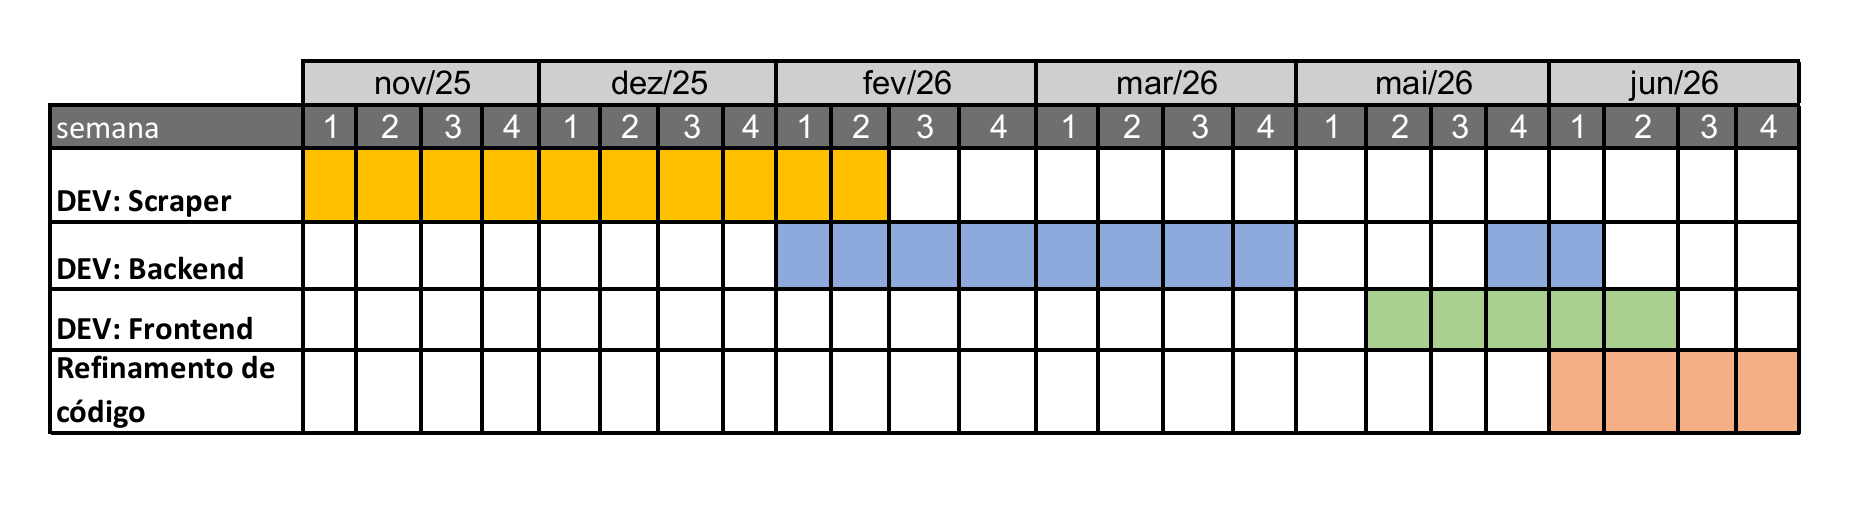
\includegraphics[width=1\linewidth]{figs/cronogramaDesenvolvimento.png}
    \caption{Cronograma de desenvolvimento}
    \label{fig:placeholder}
\end{figure}

A ideia do cronograma de desenvolvimento foi seguir a divisão de módulos do sistema, como o módulo de scraping e indexação precisa funcionar antes do processo de busca, o desenvolvimento partiu dele. Este módulo exigiu mais tempo de desenvolvimento pois foi necessário um período de entendimento de como a ferramenta deveria operar e quais ferramentas e/ou bibliotecas poderiam ser utilizadas para atingir o objetivo de obter e indexar os documentos de forma satisfatória. Além do tempo adicional para adaptar a ferramenta a realizar o scraping especificamente ao site da prefeitura de Uberlândia, que foi usado como base para a construção da ferramenta. A base para o desenvolvimento do sistema de busca foi construída no primeiro módulo, o que facilitou o desenvolvimento dos módulos seguintes, já que eles funcionam como consumidores do trabalho realizado pelo primeiro módulo e possuem baixa complexidade, tanto na API quanto no módulo de frontend, estes exigiram menor tempo de desenvolvimento.

\section{Requisitos funcionais - RF}

%<Nesta seção, apresente todos os requisitos funcionais, ou casos de uso, do sistema. Em sistemas grandes é comum haver muitos casos de uso e, para facilitar a visualização deste documento, você pode agrupá-los em subseções de casos de uso correlacionados. Os nomes das subseções devem ser únicos e pequenos (3 palavras no máximo) e podem ser formados por palavras, números e/ou abreviações. 
%Cada um dos casos de uso deve ser descrito em um bloco específico, seguindo o modelo descrito abaixo. O identificador do bloco deve conter o número do caso de uso (por exemplo, [RF001]) e o seu nome. Se os casos de uso forem agrupados em subseções específicas, a numeração deles deve ser reiniciada a cada subseção (dentro de uma mesma subseção, todo caso de uso deve ter um número de identificação único).
%Quando a primeira versão deste documento for disponibilizada para a equipe de desenvolvimento, os nomes das subseções e os números dos casos de uso não devem ser modificados ou reaproveitados, para não invalidar referências externas feitas a eles.>


\subsection{Diagrama de Caso de Uso do sistema}

O diagrama de casos de uso abaixo apresenta as principais funcionalidades do sistema de busca em Diários Oficiais.

\begin{figure}[htp]
    \centering
    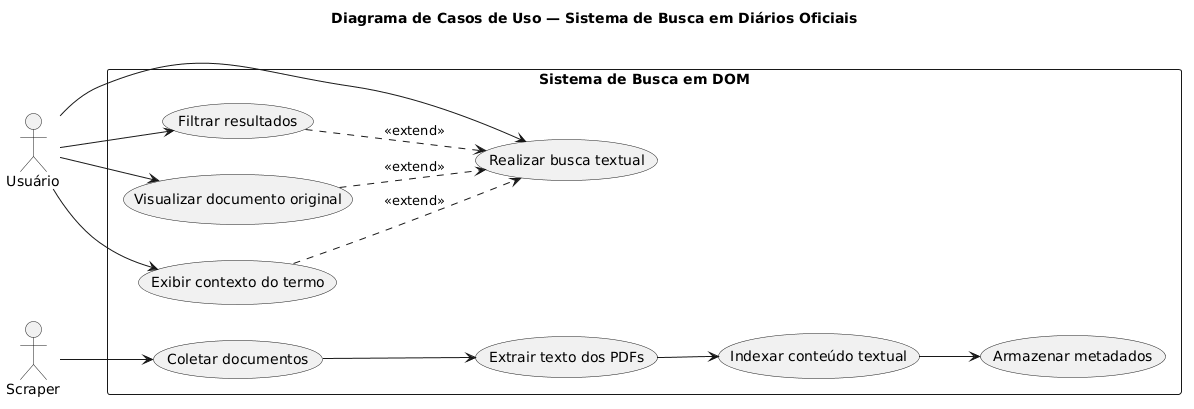
\includegraphics[width=1\linewidth]{figs/useCase.png}
    \caption{Diagrama de caso de uso do sistema}
    \label{fig:placeholder}
\end{figure}

% <Nesta seção, apresente a descrição do diagrama de caso de uso que foi levantado para o sistema>

%\begin{figure}[!ht]
%    \centering
%	\includegraphics[width=1.0\linewidth]{figs/CasodeUso.png}
%	\caption[Exemplo Diagrama de Caso de Uso do Sistema.]{Exemplo Diagrama de Caso de Uso do Sistema.}
%	\label{fig:casodeuso}
%\end{figure}

\subsection{Descrição dos Cenários dos Casos de Uso}

\subsubsection{[RF001] Realizar coleta de documentos}
\begin{itemize}
   \item \textbf{Descrição:} O sistema deve ser capaz de acessar o site da prefeitura e realizar o download dos arquivos PDF do Diário Oficial disponíveis.
   \item \textbf{Ator:} Módulo de scraping
   \item \textbf{Prioridade:} Essencial
   \item \textbf{Entradas e pré condições:} O site da prefeitura deve estar acessível e/ou o diretório contendo os arquivos para indexação.
   \item \textbf{Saídas e pós condições:} Base de dados atualizada.
   \item \textbf{Fluxo de eventos principal}
    %<Descreva aqui o fluxo de eventos principal que ocorre durante a execução do caso de uso.>
    %\begin{enumerate}
    %    \item O caso de uso inicia quando o ator fulano solicita o serviço
    %    \item Clicar em ...
    %    \item ....
    %\end{enumerate}
   %\item \textbf{Fluxos secundários} (alternativos e de exceção)
   % \begin{enumerate}
   %     \item Caso ocorra isto 
   %     \item Fazer aquilo ...
   %     \item ....
   % \end{enumerate}
 \end{itemize}

\subsubsection{[RF002] Extrair texto dos documentos}
\begin{itemize}
   \item \textbf{Descrição:} O sistema deve extrair o conteúdo textual dos arquivos PDF coletados.
   \item \textbf{Ator:} Módulo de scraping
   \item \textbf{Prioridade:} Essencial
   \item \textbf{Entradas e pré condições:} Documentos devem estar acessíveis para leitura e estruturados de forma que possibilite a extração textual.
   \item \textbf{Saídas e pós condições:} Base de dados atualizada.
   \item \textbf{Fluxo de eventos principal}
    %<Descreva aqui o fluxo de eventos principal que ocorre durante a execução do caso de uso.>
    %\begin{enumerate}
    %    \item O caso de uso inicia quando o ator fulano solicita o serviço
    %    \item Clicar em ...
    %    \item ....
    %\end{enumerate}
   \item \textbf{Fluxos secundários} (alternativos e de exceção)
    %\begin{enumerate}
    %    \item Caso ocorra isto 
    %    \item Fazer aquilo ...
    %    \item ....
    %\end{enumerate}
 \end{itemize}
 
\subsubsection{[RF003] Indexar o conteúdo textual}
\begin{itemize}
   \item \textbf{Descrição:} O sistema deve armazenar e indexar o texto extraído utilizando um mecanismo de busca textual.
   \item \textbf{Ator:} Módulo de scraping
   \item \textbf{Prioridade:} Essencial
   \item \textbf{Entradas e pré condições:} O conteúdo textual do documento deve ser obtido.
   \item \textbf{Saídas e pós condições:} Base de dados atualizada.
   \item \textbf{Fluxo de eventos principal}
    %<Descreva aqui o fluxo de eventos principal que ocorre durante a execução do caso de uso.>
    %\begin{enumerate}
    %    \item O caso de uso inicia quando o ator fulano solicita o serviço
    %    \item Clicar em ...
    %    \item ....
    %\end{enumerate}
   \item \textbf{Fluxos secundários} (alternativos e de exceção)
    %\begin{enumerate}
    %    \item Caso ocorra isto 
    %    \item Fazer aquilo ...
    %    \item ....
    %\end{enumerate}
 \end{itemize}

\subsubsection{[RF004] Armazenar metadados dos documentos}
\begin{itemize}
   \item \textbf{Descrição:} O sistema deve armazenar informações associadas aos documentos, como data, nome, número de página e origem do documento.
   \item \textbf{Ator:} Módulo de scraping
   \item \textbf{Prioridade:} Essencial
   \item \textbf{Entradas e pré condições:} O nome e data do documento devem ser obtidos.
   \item \textbf{Saídas e pós condições:} Base de dados atualizada.
   \item \textbf{Fluxo de eventos principal}
    %<Descreva aqui o fluxo de eventos principal que ocorre durante a execução do caso de uso.>
    %\begin{enumerate}
    %    \item O caso de uso inicia quando o ator fulano solicita o serviço
    %    \item Clicar em ...
    %    \item ....
    %\end{enumerate}
   \item \textbf{Fluxos secundários} (alternativos e de exceção)
    %\begin{enumerate}
    %    \item Caso ocorra isto 
    %    \item Fazer aquilo ...
    %    \item ....
    %\end{enumerate}
 \end{itemize}

\subsubsection{[RF005] Disponibilizar API de consulta}
\begin{itemize}
   \item \textbf{Descrição:} O sistema deve disponibilizar uma API REST que permita a consulta dos documentos indexados.
   \item \textbf{Ator:} Módulo de backend
   \item \textbf{Prioridade:} Essencial
   \item \textbf{Entradas e pré condições:} A base de dados indexada deve estar acessível.
   \item \textbf{Saídas e pós condições:} Serviço de consulta disponível.
   \item \textbf{Fluxo de eventos principal}
    %<Descreva aqui o fluxo de eventos principal que ocorre durante a execução do caso de uso.>
    %\begin{enumerate}
    %    \item O caso de uso inicia quando o ator fulano solicita o serviço
    %    \item Clicar em ...
    %    \item ....
    %\end{enumerate}
   \item \textbf{Fluxos secundários} (alternativos e de exceção)
    %\begin{enumerate}
    %    \item Caso ocorra isto 
    %    \item Fazer aquilo ...
    %    \item ....
    %\end{enumerate}
 \end{itemize}

\subsubsection{[RF006] Realizar busca textual}
\begin{itemize}
   \item \textbf{Descrição:} O sistema deve permitir a busca por palavras-chave no conteúdo dos documentos indexados.
   \item \textbf{Ator:} Módulo de backend
   \item \textbf{Prioridade:} Essencial
   \item \textbf{Entradas e pré condições:} A base de dados indexada deve estar acessível e as requisições devem estar corretamente formatadas.
   \item \textbf{Saídas e pós condições:} Listagem de documentos que correspondem a busca realizada.
   \item \textbf{Fluxo de eventos principal}
    %<Descreva aqui o fluxo de eventos principal que ocorre durante a execução do caso de uso.>
    %\begin{enumerate}
    %    \item O caso de uso inicia quando o ator fulano solicita o serviço
    %    \item Clicar em ...
    %    \item ....
    %\end{enumerate}
   \item \textbf{Fluxos secundários} (alternativos e de exceção)
    %\begin{enumerate}
    %    \item Caso ocorra isto 
    %    \item Fazer aquilo ...
    %    \item ....
    %\end{enumerate}
 \end{itemize}

 \subsubsection{[RF007] Filtrar resultados de busca}
\begin{itemize}
   \item \textbf{Descrição:} O sistema deve permitir a aplicação de filtros nos resultados de busca, como data, período e edição.
   \item \textbf{Ator:} Módulo de backend
   \item \textbf{Prioridade:} Essencial
   \item \textbf{Entradas e pré condições:} A base de dados indexada deve estar acessível e as requisições devem estar corretamente formatadas.
   \item \textbf{Saídas e pós condições:} Listagem de documentos que correspondem a filtragem realizada.
   \item \textbf{Fluxo de eventos principal}
    %<Descreva aqui o fluxo de eventos principal que ocorre durante a execução do caso de uso.>
    %\begin{enumerate}
    %    \item O caso de uso inicia quando o ator fulano solicita o serviço
    %    \item Clicar em ...
    %    \item ....
    %\end{enumerate}
   \item \textbf{Fluxos secundários} (alternativos e de exceção)
    %\begin{enumerate}
    %    \item Caso ocorra isto 
    %    \item Fazer aquilo ...
    %    \item ....
    %\end{enumerate}
 \end{itemize}

 \subsubsection{[RF008] Exibir resultados da busca}
\begin{itemize}
   \item \textbf{Descrição:} O sistema deve apresentar ao usuário os documentos encontrados contendo o termo pesquisado.
   \item \textbf{Ator:} Módulo de frontend
   \item \textbf{Prioridade:} Essencial
   \item \textbf{Entradas e pré condições:} A API de busca deve estar acessível.
   \item \textbf{Saídas e pós condições:} Listagem visual de documentos que correspondem a filtragem realizada.
   \item \textbf{Fluxo de eventos principal}
    %<Descreva aqui o fluxo de eventos principal que ocorre durante a execução do caso de uso.>
    %\begin{enumerate}
    %    \item O caso de uso inicia quando o ator fulano solicita o serviço
    %    \item Clicar em ...
    %    \item ....
    %\end{enumerate}
   \item \textbf{Fluxos secundários} (alternativos e de exceção)
    %\begin{enumerate}
    %    \item Caso ocorra isto 
    %    \item Fazer aquilo ...
    %    \item ....
    %\end{enumerate}
 \end{itemize}

  \subsubsection{[RF009] Exibir contexto do resultado}
\begin{itemize}
   \item \textbf{Descrição:} O sistema deve mostrar um trecho do texto em que o termo pesquisado aparece.
   \item \textbf{Ator:} Módulo de frontend
   \item \textbf{Prioridade:} Importante
   \item \textbf{Entradas e pré condições:} A API de busca deve estar acessível.
   \item \textbf{Saídas e pós condições:} Listagem textual de conteúdos de documentos que correspondem a busca realizada.
   \item \textbf{Fluxo de eventos principal}
    %<Descreva aqui o fluxo de eventos principal que ocorre durante a execução do caso de uso.>
    %\begin{enumerate}
    %    \item O caso de uso inicia quando o ator fulano solicita o serviço
    %    \item Clicar em ...
    %    \item ....
    %\end{enumerate}
   \item \textbf{Fluxos secundários} (alternativos e de exceção)
    %\begin{enumerate}
    %    \item Caso ocorra isto 
    %    \item Fazer aquilo ...
    %    \item ....
    %\end{enumerate}
 \end{itemize}

\subsubsection{[RF010] Permitir acesso ao documento original}
\begin{itemize}
   \item \textbf{Descrição:} O sistema deve permitir que o usuário acesse ou visualize o documento PDF original correspondente ao resultado da busca.
   \item \textbf{Ator:} Módulo de frontend
   \item \textbf{Prioridade:} Essencial
   \item \textbf{Entradas e pré condições:} Os documentos devem estar disponíveis no serviço de hospedagem.
   \item \textbf{Saídas e pós condições:} Acesso aos documentos recuperados pela busca
   \item \textbf{Fluxo de eventos principal}
    %<Descreva aqui o fluxo de eventos principal que ocorre durante a execução do caso de uso.>
    %\begin{enumerate}
    %    \item O caso de uso inicia quando o ator fulano solicita o serviço
    %    \item Clicar em ...
    %    \item ....
    %\end{enumerate}
   \item \textbf{Fluxos secundários} (alternativos e de exceção)
    %\begin{enumerate}
    %    \item Caso ocorra isto 
    %    \item Fazer aquilo ...
    %    \item ....
    %\end{enumerate}
 \end{itemize}

\section{Requisitos Não Funcionais - RNF}

%<Esta seção deve conter os requisitos não funcionais do sistema. Para uma melhor organização deste documento, utilize as subseções abaixo para agrupar os requisitos não funcionais relacionados. Naturalmente, o número e tipo de subseções utilizadas depende do sistema que está sendo especificado e não é preciso utilizar todas elas. Simplesmente elimine as subseções para as quais não for encontrado nenhum requisito.
%Os requisitos não funcionais devem ser identificados com um identificador único, da mesma maneira que os requisitos funcionais (casos de uso). Inicie a numeração com o identificador NF001 e prossiga incrementando os números a medida que forem surgindo novos requisitos não funcionais. Reinicie a numeração em cada subseção. Forneça também um nome para o requisito, como foi feito para os requisitos funcionais.
%Descreva o requisito, assinale a sua prioridade e, em seguida, caso o requisito esteja relacionado a um caso de uso ou a um grupo de casos de uso específicos, utilize o campo “Caso(s) de uso associado(s):” para identificar o(s) caso(s) de uso correspondente(s). Se for um requisito não funcional do sistema como um todo, esse campo não precisa ser utilizado.>

\subsection{[RNF001] Desempenho}
 \begin{itemize}
    \item \textbf{Descrição:} O sistema deve retornar os resultados das consultas em tempo adequado, permitindo buscas eficientes mesmo com grande quantidade de documentos indexados.
    \item \textbf{Prioridade:} Importante.
    \item \textbf{Caso(s) de uso associado(s):} RF006, RF008
\end{itemize}

\subsection{[RNF002] Usabilidade}
 \begin{itemize}
    \item \textbf{Descrição:} A interface web deve ser simples e intuitiva, permitindo que usuários realizem buscas sem necessidade de treinamento prévio.
    \item \textbf{Prioridade:} Importante.
    \item \textbf{Caso(s) de uso associado(s):} RF006, RF008, RF009, RF010
\end{itemize}


\subsection{[RNF003] Escalabilidade}
\begin{itemize}
    \item \textbf{Descrição:} A arquitetura do sistema deve permitir a expansão para indexar documentos de outras prefeituras ou fontes de Diários Oficiais.
    \item \textbf{Prioridade:} Desejável.
    \item \textbf{Caso(s) de uso associado(s):} RF001, RF003, RF004, RF005
\end{itemize}


\subsection{[RNF004] Manutenabilidade}
\begin{itemize}
    \item \textbf{Descrição:} O sistema deve possuir uma arquitetura modular que facilite manutenção, atualização e inclusão de novas funcionalidades.
    \item \textbf{Prioridade:} Desejável.
    \item \textbf{Caso(s) de uso associado(s):}
\end{itemize}

\subsection{[RNF005] Disponibilidade}
\begin{itemize}
    \item \textbf{Descrição:} A API e a interface web devem estar disponíveis para acesso sempre que o sistema estiver em operação.
    \item \textbf{Prioridade:} Essencial.
    \item \textbf{Caso(s) de uso associado(s):} RF005, RF006, RF007, RF008, RF009, RF010
\end{itemize}

\subsubsection{[RNF006] Compatibilidade}
\begin{itemize}
    \item \textbf{Descrição:} A aplicação web deve ser compatível com os principais navegadores modernos. 
    \item \textbf{Prioridade:} Essencial
    \item \textbf{Caso(s) de uso associado(s):} RF008, RF009, RF010
\end{itemize}

\subsubsection{[RNF007] Portabilidade}
\begin{itemize}
    \item \textbf{Descrição:} O sistema deve ser capaz de ser executado em diferentes ambientes computacionais compatíveis com as tecnologias utilizadas.
    \item \textbf{Prioridade:} Importante.
    \item \textbf{Caso(s) de uso associado(s):} RF010
\end{itemize}

\subsubsection{[RNF008] Confiabilidade}
\begin{itemize}
    \item \textbf{Descrição:} O sistema deve garantir a integridade dos dados armazenados no banco de dados.
    \item \textbf{Prioridade:} Essencial.
    \item \textbf{Caso(s) de uso associado(s):} RF010
\end{itemize}

\section{Protótipos das interfaces com usuários}
A figura X ilustra um esboço do layout da pagina de buscas, a ideia foi manter todo o conteúdo necessário em somente uma página, com o componente de formulário de pesquisa sendo o elemento central. Além de uma exibição do documento mais recente.

\begin{figure} [htbp!]
    \centering
    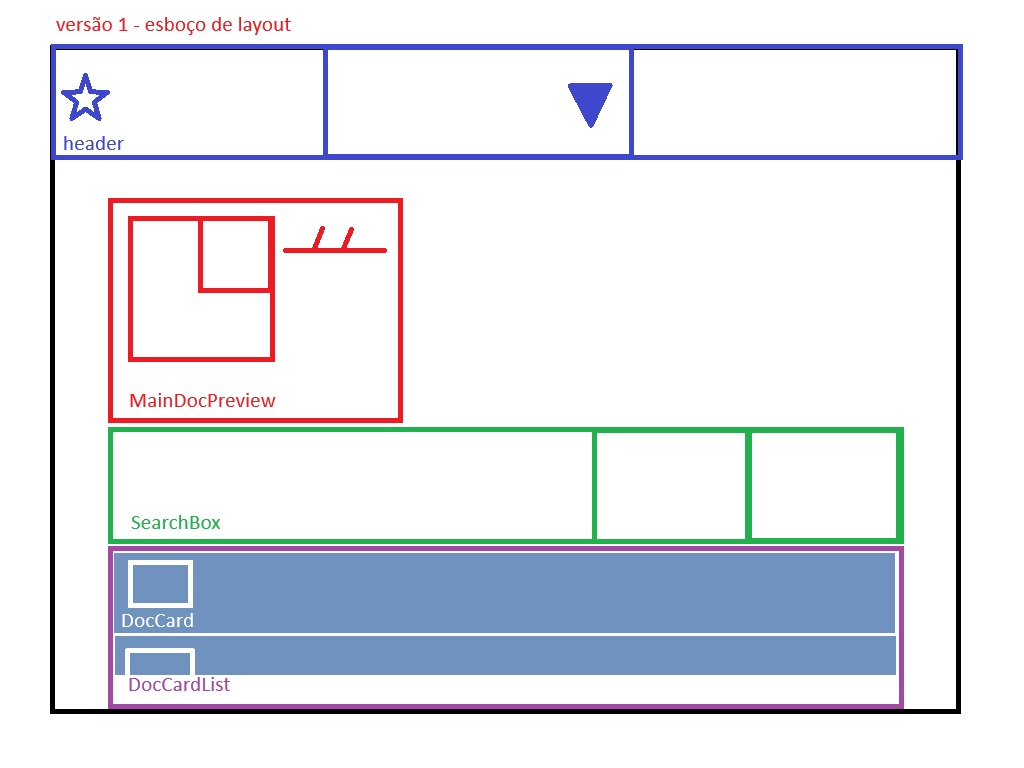
\includegraphics[width=0.7\linewidth]{figs/esboco-layout1.jpg}
    \caption{Protótipo inicial}
    \label{fig:placeholder}
\end{figure}

Já a figura X exibe uma captura da tela em estágio de desenvolvimento, a estrutura segue o que foi definido no esboço inicial e serviu como ponto de partida para refinamento final. Neste estágio o sistema já estava operacional para realização de buscas e exibição de resultados, porém sua estrutura visual ainda não estava preparada para ter responsividade para o acesso através de dispositivos móveis. 

\begin{figure} [htbp!]
    \centering
    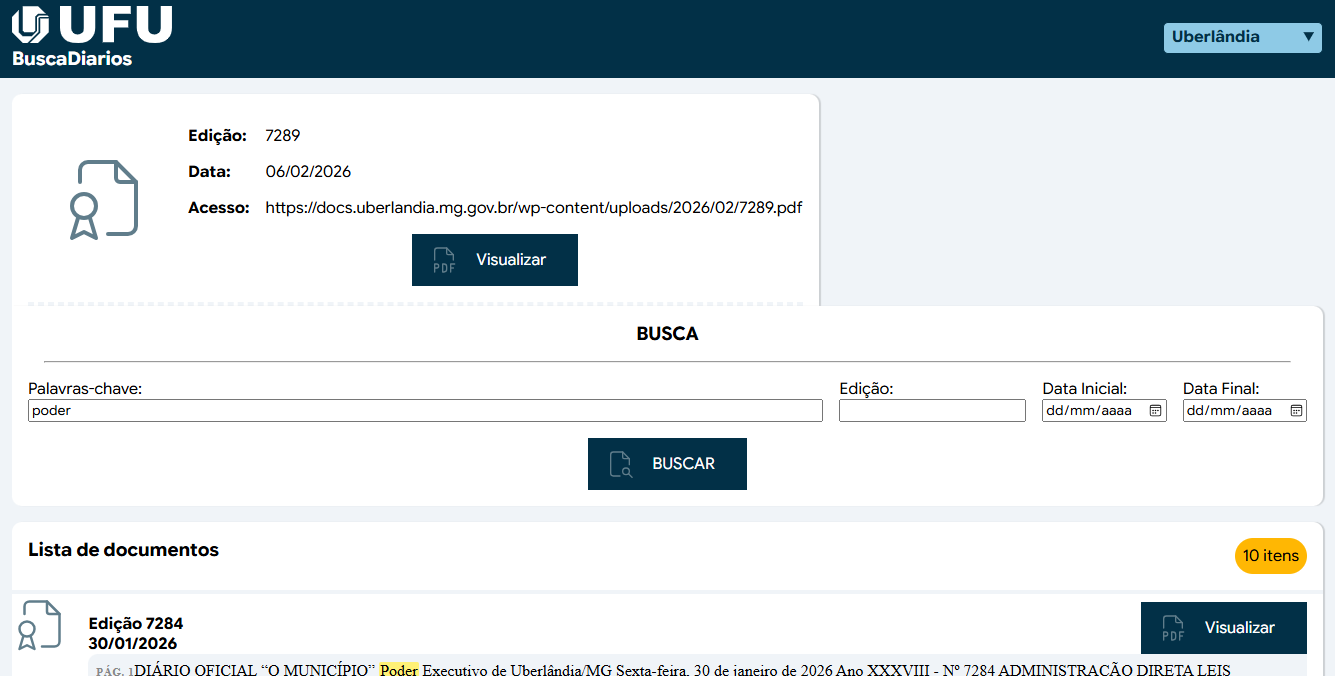
\includegraphics[width=0.7\linewidth]{figs/diariosScraperUI.png}
    \caption{Versão inicial operável}
    \label{fig:placeholder}
\end{figure}

Por fim, na captura da figura X contém o sistema em estágios finais de desenvolvimento, com refinamentos na exibição de resultados e com responsividade melhorada para permitir o acesso da página através de dispositivos móveis.

\begin{figure} [htbp!]
    \centering
    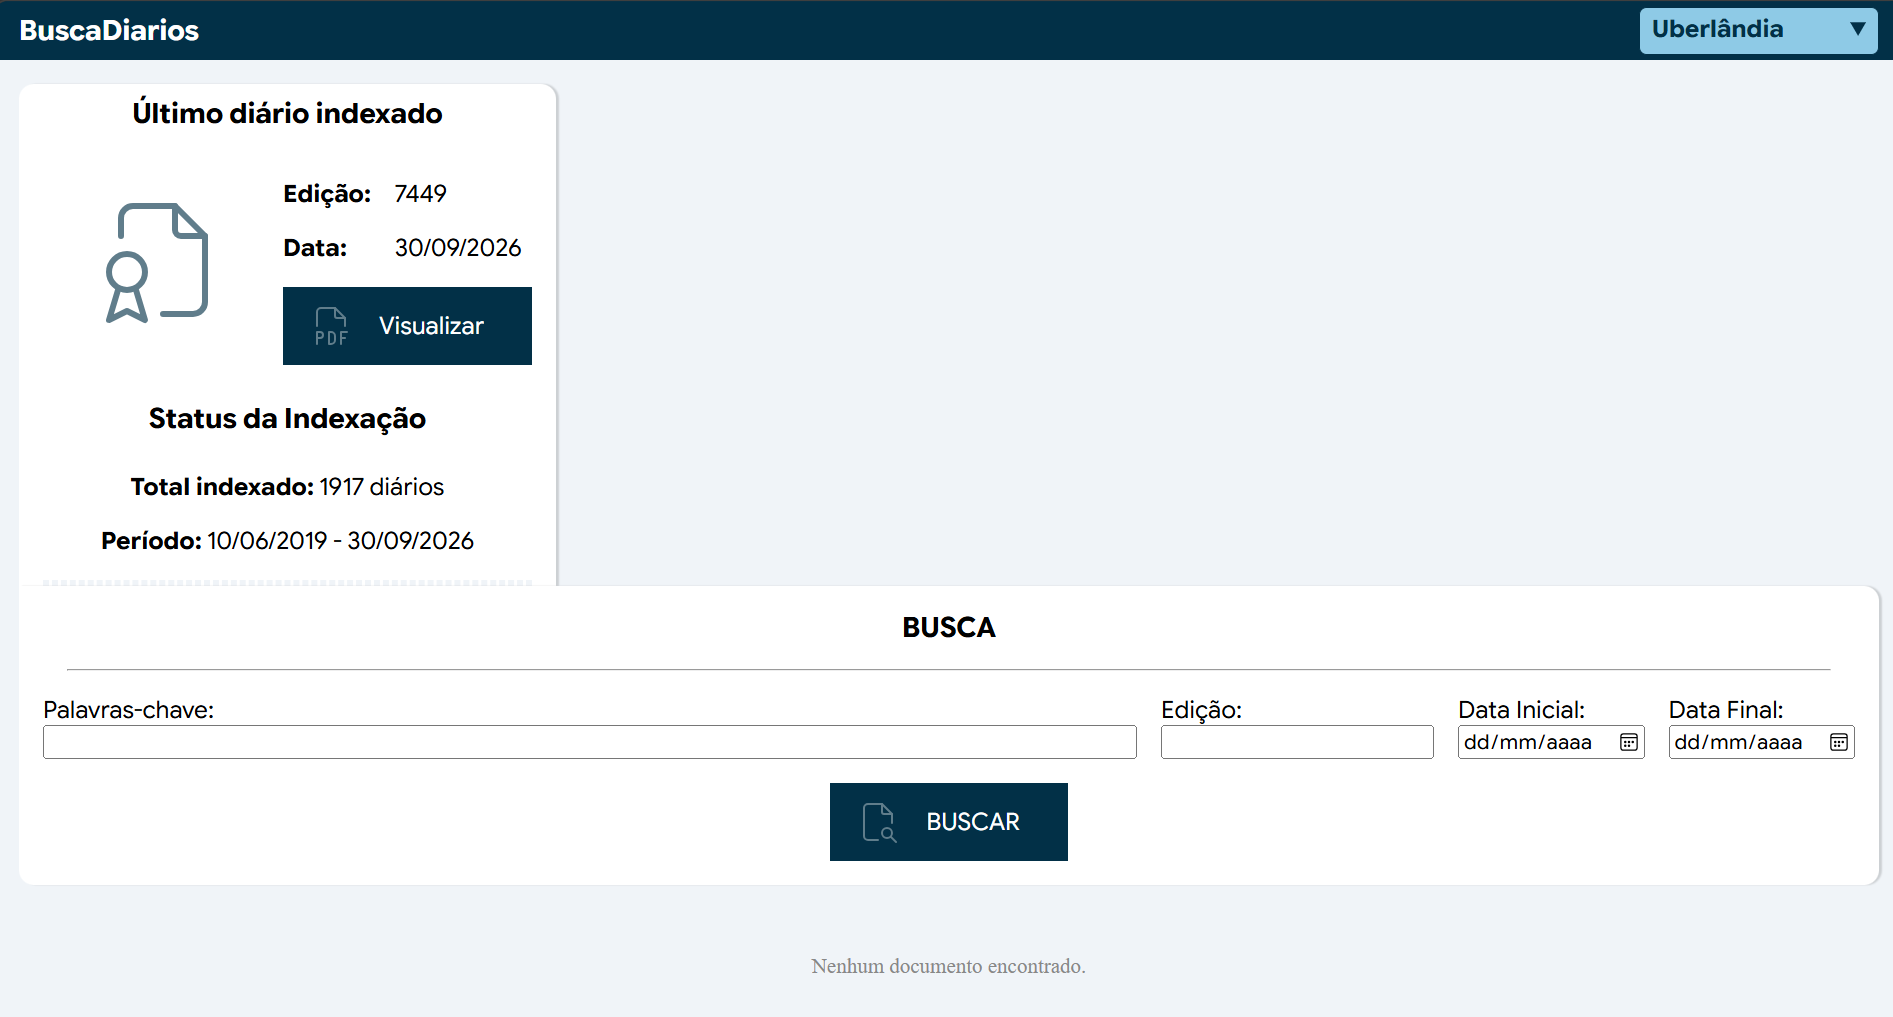
\includegraphics[width=0.7\linewidth]{figs/prints/versao_final.png}
    \caption{Versão final}
    \label{fig:placeholder}
\end{figure}

%<Esta seção deve conter desenhos ou rascunhos das telas do sistema que forem necessários ou convenientes para esclarecer algum dos requisitos do sistema. Para sistemas que possuem protótipos ou versões já desenvolvidas é possível capturar as telas e apresentar figuras das mesmas.
%Use nomes e/ou números para identificar cada interface e descreva-as em seções independentes.>

\section{Considerações Sobre o Capítulo}
Neste capítulo foram apresentados os requisitos do sistema de busca em Diários Oficiais Municipais, incluindo a arquitetura geral da solução, a caracterização dos usuários, os requisitos funcionais e não funcionais e os casos de uso identificados. A especificação apresentada estabelece uma base para o desenvolvimento e avaliação da solução proposta, permitindo que as etapas de implementação sejam conduzidas de forma estruturada e alinhada aos objetivos do trabalho